\chapter{Il Livello di Trasporto}
\thispagestyle{chapterInit}
\paragraph{Obbiettivi}
    \begin{itemize}
        \item Capire i principi che sono alla base dei servizi di livello di trasporto:
            \subitem Multiplexing/de-multiplexing
            \subitem Trasferimento dati affidabile
            \subitem Controllo di flusso
            \subitem Controllo di congestione
        \item Descrivere i protocolli del livello di trasporto di Internet:
            \subitem TCP: Trasposto orientato alla connessione
            \subitem Controllo di congestione TCP
            \subitem UDP: Trasporto non orientato alla connessione
    \end{itemize}
\section{Servizi a livello di trasporto}
    \paragraph{Introduzione} I \textbf{protocolli di trasporto} forniscono la comunicazione logica tra processi applicativi di host diversi. I protocolli di trasporto vengono eseguiti negli host "terminali" ovvero quelli che generano o consumano i dati. Dal lato di inviante il protocollo di trasporto divide in diversi segmenti i dati ricevuti dal livello di applicazione e li invia al livello di rete. Dal lato di ricevente il protocollo di trasporto riassembla i segmenti ricevuti e li invia al livello di applicazione.
    \paragraph{TCP} Il \textbf{TCP} (Transmission Control Protocol) è un protocollo di trasporto orientato alla connessione. Il TCP fornisce un trasferimento affidabile dei dati, controllo di flusso e controllo di congestione.
    \paragraph{UDP} L'\textbf{UDP} (User Datagram Protocol) è un protocollo di trasporto non orientato alla connessione. L'UDP non fornisce trasferimento affidabile dei dati, controllo di flusso e controllo di congestione.
    \paragraph{Servizi non disponibili} Al momento in internet non è disponibile un servizio di garanzia su ritardi (latenza), e non è disponibile un servizio di garanzia sulla banda (velocità di trasferimento).
\section{Multiplexing e De-multiplexing}
    \paragraph{Introduzione} Il \textbf{multiplexing} è il processo di invio di dati da più socket a un'unica connessione, per identificare il socket di destinazione si utilizza un \textbf{port number}. Il \textbf{de-multiplexing} è il processo di invio dei dati ricevuti al socket corretto in base al port number.
    \subsection{De-multiplexing}
        \paragraph{Come funziona} In primo luogo quando l'\textit{host} riceve un segmento IP contenente: IP del mittente, IP del destinatario, protocollo di trasporto, porta di destinazione e porta di sorgente. L'\textit{host} utilizza l'indirizzo IP del destinatario e la porta di destinazione per inviare il segmento al processo corretto.
        \subsubsection{De-multiplexing senza connessione}
            Per eseguire il de-multiplexing senza connessione si crea un socket per ricevere i dati. Il socket è ora associato a una porta ed a un indirizzo IP. Quando l'\textit{host} riceve il segmento \texttt{UDP}, viene controllato che il numero di porta di destinazione sia uguale alla porta del socket. Se il numero di porta non corrisponde il segmento viene scartato. Se invece il numero di porta corrisponde il segmento viene inviato al processo associato al socket.
            \begin{figure}[H]
                \centering
                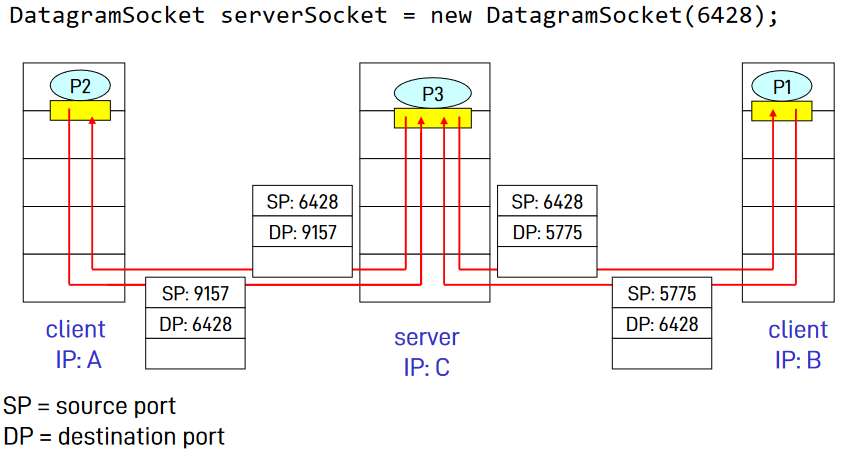
\includegraphics[width=0.5\textwidth]{03/DemultiplexingSenzaConnessione.png}
                \caption{De-multiplexing senza connessione}
            \end{figure}
        \subsubsection{De-multiplexing orientato alla connessione}
            Quando si utilizza un protocollo orientato alla connessione (\texttt{TCP}), il processo di de-multiplexing è leggermente diverso. Il socket infatti è costituito da quattro parametri: indirizzo IP del mittente, indirizzo IP del destinatario, numero di porta di sorgente e numero di porta di destinazione. Quando l'\textit{host} riceve un segmento \texttt{TCP} controlla che i quattro parametri del socket corrispondano ai quattro parametri del segmento. Se i parametri non corrispondono il segmento viene scartato, altrimenti viene inviato al processo associato al socket. Un \textit{host} può supportare più socket contemporaneamente purché cambi almeno uno dei quattro parametri, inoltre i \textit{web server} sono un chiaro esempio di applicazione che utilizza più socket contemporaneamente (su \texttt{HTTP/1.0} un socket per ogni richiesta).\footnote{Se viene allocata una porta ad una connessione, la porta non può essere utilizzata da altre connessioni, quindi nel caso di un \textit{web server} è vero che questo ascolta sulla porta 80, ma quando un client si connette al server, il server apre un socket con una porta dinamica.}
            \begin{figure}[H]
                \centering
                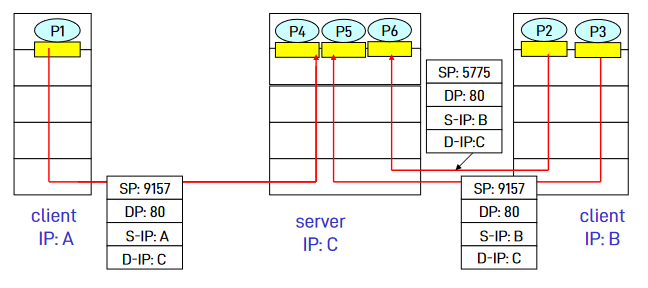
\includegraphics[width=0.5\textwidth]{03/DemultiplexingConConnessione.png}
                \caption{De-multiplexing orientato alla connessione}
            \end{figure}
    \subsection{Porte \texttt{TCP}-\texttt{UDP}}
        La destinazione finale di un segmento non è un host ma un processo. L'interfaccia tra l'applicazione e il livello di trasporto è chiamata \textbf{socket} o \textbf{porta} (nel caso di \texttt{UDP} e \texttt{TCP}). Un \textbf{socket} è un indirizzo IP e un numero di porta. Un \textbf{port number} è un numero a 16 bit che identifica un processo all'interno di un host. Esiste una mappatura biunivoca tra un \textbf{port number} e un processo. I servizi standard utilizzano porte ben note con valori tra 0 e 1023. I processi non-standard e le connessioni in ingresso a un client usano numeri fino a 25535 (16 bit).
        \paragraph{Numeri di porte}
            I numeri di porta si classificano come segue:
            \begin{description}
                \item[Statici] Per i servizi standard, es. HTTP (80), FTP (21), SSH (22), Telnet (23), SMTP (25), POP3 (110), IMAP (143), HTTPS (443), ecc.
                \item[Dinamici] (o "ephemeral") per le connessioni in uscita o per porte allocate dinamicamente, es. client web, client FTP, client SSH, client Telnet, client SMTP, client POP3, client IMAP, client HTTPS, ecc.
            \end{description}
            Inoltre è importante dire che le porte di sorgente e di destinazione non sono le stesse in quanto la porta di sorgente è una porta dinamica assegnata dal sistema operativo.
\section{Trasporto senza connessione: \texttt{UDP}}
    \paragraph{Caratteristiche} L'\textbf{UDP} (User Datagram Protocol) è un protocollo di trasporto senza connessione, offre un servizio \textit{best effort} e non fornisce garanzie di consegna, ordine o duplicazione dei dati. Questo in quanto non ha \textit{handshake} iniziale e non mantiene alcuno stato di connessione. 
    \paragraph{Perché esiste \texttt{UDP}} Non richiede di stabilire una connessione, è semplice e veloce, Header di segmento corti, senza controllo di congestione.
    \subsection{Header}
        \begin{figure}[H]
            \centering
            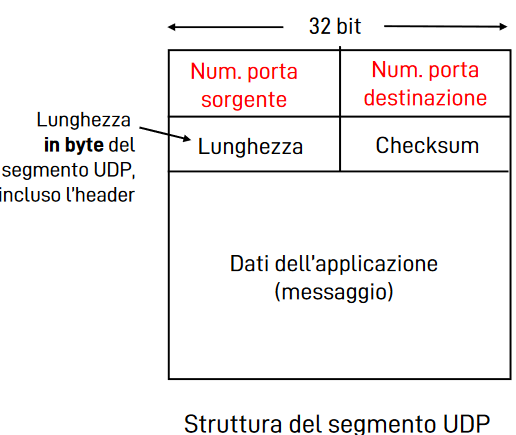
\includegraphics[width=0.3\textwidth]{03/UDPHeader.png}
            \caption{Header di un segmento UDP}
        \end{figure}
        \begin{description}
            \item[Porta di sorgente] Numero di porta del processo mittente.
            \item[Porta di destinazione] Numero di porta del processo destinatario.
            \item[Lunghezza] Lunghezza del segmento in byte.
            \item[Checksum] Utilizzato per rilevare errori nel segmento.
        \end{description}
        \subsubsection{Checksum}
            Il checksum è un campo a 16 bit che viene utilizzato per rilevare errori nel segmento. Questo viene calcolato da entrambe le parti: viene trattato il contenuto come una sequenza di $ 16 $ bit e si sommano tutti i bit (se presente riporto questo viene sommato a sua volta) e viene eseguito il complemento a 1. Il mittente invia il checksum calcolato nel segmento e il ricevente calcola il checksum del segmento ricevuto e lo confronta con il checksum ricevuto. Se i due checksum non corrispondono il segmento viene scartato.
\section[trasferimento dati affidabile]{Principi del trasferimento dati affidabile}
    \subsection{\texttt{ARQ}}
        \textbf{\texttt{ARQ}} o \textit{Automatic Repeat reQuest} è una classe di protocolli che "cercano" di recuperare i segmenti persi o danneggiati. Questa classe usa dei pacchetti speciali per notificare al mittente che un segmento è stato perso o danneggiato. Questi pacchetti speciali sono chiamati \texttt{ACK} (Acknowledgement) e \texttt{NACK} (Negative Acknowledgement).
        \paragraph{Esempi di protocolli basati su \texttt{ARQ}} \begin{itemize}
            \item \textit{Stop-and-Wait}
            \item \textit{Go-Back-N}
            \item \textit{Selective Repeat}
            \item \texttt{TCP}
            \item il protocollo \texttt{MAC} (al livello 2) dei sistemi \texttt{WiFi}
        \end{itemize}
    \subsection{\textit{Stop-and-Wait}}
        Nel protocollo \textit{Stop-and-Wait} il mittente invia una \texttt{PDU} e ne mantiene una copia in memoria, imposta dunque un \textit{timeout} su quel \texttt{PDU}. Attende poi un \texttt{ACK} dal ricevente, se non riceve l'\texttt{ACK} entro il \textit{timeout} invia nuovamente la \texttt{PDU}. Se invece riceve l'\texttt{ACK} controlla che questo non contenga errori, che sia il numero di sequenza corretto e che sia per la \texttt{PDU} inviata. Se tutto è corretto invia la prossima \texttt{PDU}. Il ricevente quando riceve una \texttt{PDU} controlla che il numero di sequenza sia corretto e che la \texttt{PDU} non abbia errori, se tutto è corretto invia un \texttt{ACK} al mittente, de-capsula la \texttt{PDU} ai livelli superiori. Se sono presenti errori nella \texttt{PDU} il ricevente esegue il \textit{drop} della \texttt{PDU}.
        \subsubsection{Efficienza dello \textit{Stop-and-Wait}}
            Assumendo una banda $ R = 1 G-bit/s, 15ms $ di ritardo di propagazione, lunghezza del messaggio $ L = 8000bit $, allora il tempo di trasmissione sarà: $T_{trans} = \frac{L}{R} = \frac{80000}{10^9} = 8\mu s$. Mentre il \textit{throughput} percepito a livello applicativo sarà: $ \frac{L}{T_{trans}+RTT}= \frac{8000}{8\mu s + 30ms} = 33 Kbps $.\footnote{Aggiungiamo della formula il \texttt{RTT} ovvero il \textit{Round Trip Time} che è il tempo che impiega un pacchetto per andare dal mittente al ricevente e ritornare indietro, nel nostro caso lo aggiungiamo per il pacchetto di \texttt{ACK} ed è di $ 30ms $.} Dunque anche se la nostra banda è di $ 1 Gbps $ il \textit{throughput} percepito a livello applicativo è di $ 33 Kbps $, l'efficienza dunque è: $ \frac{T_{trans}}{T_{trans}+RTT} = \frac{0.008}{0.008+30} = 0.00027 $ ovvero $ 0.027\% $.
    \subsection{Protocolli con \textit{pipelining}}
        I protocolli con \textit{pipelining} permettono di inviare più segmenti successivi senza attendere l'\texttt{ACK} del segmento precedente, si allarga dunque il range dei pacchetti di sequenza accettabili. Questo permette di aumentare l'efficienza del trasferimento dati. Esempio di protocolli con \textit{pipelining} sono \textit{Go-Back-N} e \textit{Selective Repeat}.
        \subsubsection{\textit{Throughput} in presenza di \textit{pipelining}}
            Assumiamo la stessa situazione precedente ed un \textit{pipelining} di $ N = 3 $ allora il \textit{throughput} sarà: $ \frac{3L}{T_{trans}+RTT} = \frac{24000}{8\mu s + 30ms} = 100 Kbps $, questo è un miglioramento del $ 300\% $ rispetto allo \textit{Stop-and-Wait}. In generale il \textit{throughput} rispetto al \textit{pipelining} con $ N $ segmenti in parallelo è: $ \frac{N \cdot L}{RTT + T_{trans}} $. Il parametro $ N $ è detto \textit{window size} o "dimensione della finestra".
        \subsubsection{Definizioni}
            \begin{description}
                \item[Finestra di trasmissione $W_T$] Insieme di \texttt{PDU} che il mittente può inviare senza attendere un \texttt{ACK} del ricevente.
                    \subitem Grande al massimo come la memoria allocata dal sistema operativo.
                    \subitem $\left|W_T\right|$ indica la dimensione della finestra.
                \item[Finestra di ricezione $W_R$] Insieme di \texttt{PDU} che il ricevente può ricevere può accettare e memorizzare.
                    \subitem Grande al massimo come la memoria allocata dal sistema operativo.
                \item[Puntatore \textit{low} $W_{LOW}$] Indica il primo segmento della finestra di trasmissione $W_T$.
                \item[Puntatore \textit{high} $W_{HIGH}$] Indica l'ultimo segmento già trasmesso della finestra di trasmissione $W_T$.
            \end{description}
        
        \begin{figure}[H]
            \centering
            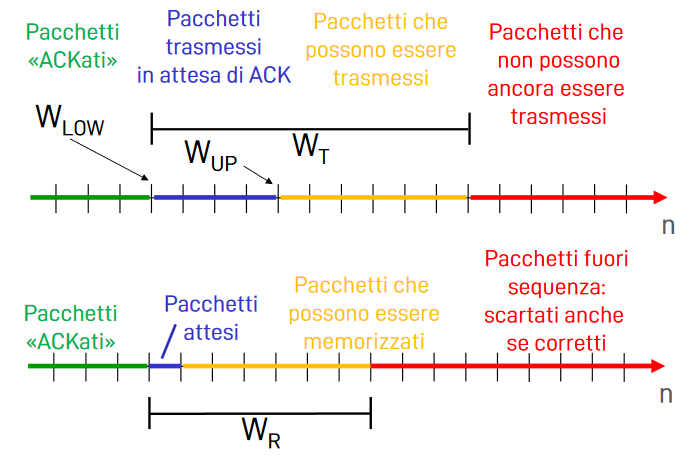
\includegraphics[width=0.5\textwidth]{03/finestrePipelining.png}
            \caption{Finestre di trasmissione e di ricezione}
        \end{figure}
        \subsubsection{\textit{Acknowledgements} - \texttt{ACK}}
            Esistono vari tipi di \texttt{ACK} a seconda del protocollo utilizzato, abbiamo dunque:
            \begin{itemize}
                \item \texttt{ACK} individuale il cui compito è quello di indicare la corretta ricezione di uno specifico pacchetto - \texttt{ACK($n$)} vuol dire ho ricevuto il pacchetto $n$.
                \item \texttt{ACK} cumulativo il cui compito è quello di indicare la corretta ricezione di tutti i pacchetti fino a quello specificato - \texttt{ACK($n$)} vuol dire ho ricevuto tutti i pacchetti fino a $n$ (escluso), mi aspetto il pacchetto $n$.
                \item \texttt{ACK} negativo o \texttt{NACK} il cui compito è quello di indicare la mancata ricezione di un pacchetto - \texttt{NACK($n$)} vuol dire non ho ricevuto il pacchetto $n$, invialo nuovamente.
                \item Esiste poi la tecnica del "\textbf{Piggybacking}", ovvero l'inserimento dell'\texttt{ACK} (di un pacchetto precedente) all'interno di un pacchetto dati successivo.
            \end{itemize}
        \subsubsection{\textit{Go-Back-N}}
            Quando si sceglie di usare il protocollo del tipo \textit{Go-Back-N} questo consiste in: il mittente invia fino ad un numero $ n $ di pacchetti senza aver ricevuto prima \texttt{ACK}, quando un pacchetto è stato ricevuto correttamente viene inviato un \texttt{ACK} cumulativo, se un pacchetto non è stato ricevuto allora i pacchetti successivi vengono scartati in attesa del pacchetto mancante. Dopo un periodo di \textit{timeout} il mittente invia nuovamente tutti i pacchetti a partire dal pacchetto mancante, basandosi sull'ultimo \texttt{ACK} ricevuto. La finestra di trasmissione $ W_T $ è dunque composta da $ n $ pacchetti e non viene spostata finché non si riceve un \texttt{ACK} cumulativo, mentre la finestra di ricezione $ W_R $ è composta da un solo pacchetto.
        \subsubsection{\textit{Selective Repeat}}
            Nel paradigma del \textit{selective repeat} vengono usati \texttt{ACK} singoli, inoltre è presente una finestra di ricezione $ W_R $ composta da $ m $ pacchetti, ciò significa che anche se un pacchetto ricevuto fuori sequenza viene ricevuto allora questo viene comunque "salvato" all'interno di un buffer in attesa del pacchetto nell'ordine corretto. Anche il mittente in caso di \texttt{ACK} fuori sequenza conserva in memoria questo dato e non lo scarta. Quello che succede se un pacchetto non viene ricevuto ma qualche pacchetto (fino a $m-1$) successivo viene ricevuto correttamente è che il mittente invia nuovamente solo il pacchetto mancante, mentre i pacchetti successivi, se sono già stati \texttt{ACK'ati}, non vengono inviati nuovamente e la trasmissione riprende dal primo pacchetto non \texttt{ACK' ato}.
        \paragraph{Spazio dei numeri di sequenza}
            Solitamente se si hanno $ k $ bit a disposizione allora si usa un periodo pari a $ 2^k $, ovvero il periodo massimo con quello spazio di bit. Le finestre di trasmissione per non avere conflitti devono avere somma inferiore al periodo, quindi $ |W_T| + |W_R| < 2^k $.
\section[Trasporto Orientato Connessione \texttt{TCP}]{Trasporto orientato alla connessione \texttt{TCP}}
    \paragraph{\texttt{TCP} - vari standard \texttt{RFC}} Il \texttt{TCP} o \textit{Transmission Control Protocol} è un protocollo di trasporto orientato alla connessione, è stato standardizzato nel \texttt{RFC 793} e successivamente aggiornato con il \texttt{RFC 1122}, \texttt{RFC 1323}, \texttt{2018}, \texttt{2581} ed è in continuo aggiornamento. Questo prevede una connessione \underline{punto-punto} tra mittente e destinatario, è presente un flusso di byte affidabile e consegnato in ordine senza limiti, è presente un meccanismo di \textit{pipelining} e di controllo di congestione per non sovraccaricare la rete. La connessione inoltre (anche se a livelli inferiori non lo è) è \textit{\underline{full-duplex}} ovvero entrambi i lati possono inviare e ricevere dati contemporaneamente. Inoltre il \texttt{TCP} è un protocollo \textit{\underline{stateful}} ovvero mantiene uno stato della connessione, infatti si dice che è orientato alla connessione. Infine ha presente un flusso controllato, il trasmettitore non può inviare dati se il ricevente non è pronto a riceverli.\newpage
    \subsection{Struttura di un pacchetto \texttt{TCP}}
        \begin{figure}[H]
            \centering
            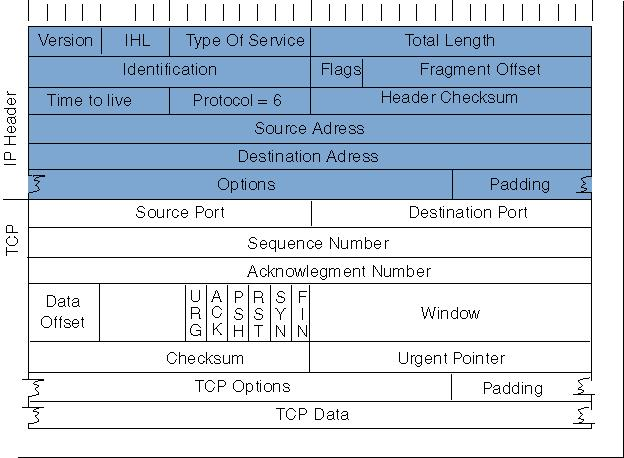
\includegraphics[width=0.45\textwidth]{03/pacchettoTCP.jpg}
            \caption{Struttura di un pacchetto \texttt{TCP}} 
            \footnote{Immagine tratta da \href{https://commons.wikimedia.org/wiki/File:Ntwk_tcp_header.jpg}{Wikimedia Commons} di Gopalpaliwal at English Wikibooks il file è rilasciato sotto licenza Creative Commons \href{https://creativecommons.org/licenses/by-sa/3.0/deed.en}{Attribution-Share Alike 3.0 Unported}.}
        \end{figure}
        Nel pacchetto \texttt{TCP} sono presenti i seguenti campi principali:
        \begin{description}
            \item[Source Port] Porta di sorgente.
            \item[Destination Port] Porta di destinazione.
            \item[Sequence Number] Numero di sequenza del primo byte del segmento.
            \item[Acknowledgement Number] Numero di sequenza del prossimo byte atteso.
            \item[Data Offset] Lunghezza dell'header in parole di 32 bit.
            \item[URG] Flag che indica la presenza di dati urgenti.
            \item[ACK] Flag che indica la presenza di un campo \texttt{ACK}.
            \item[PSH] Flag che indica che i dati devono essere passati al livello superiore.
            \item[PST] Flag che indica l'inizio di una connessione.
            \item[SYN] Flag che indica la sincronizzazione dei numeri di sequenza.
            \item[FIN] Flag che indica la chiusura della connessione.
            \item[Window] Dimensione della finestra di ricezione. (RWND)
            \item[Checksum] Utilizzato per rilevare errori nel segmento (contiene oltre ai parametri \texttt{TCP} anche i parametri \texttt{IP} come l'indirizzo IP del mittente e del destinatario, la lunghezza del segmento, il protocollo di trasporto, ecc.).
            \item[Urgent Pointer] Puntatore ai dati urgenti.
            \item[TCP Options] Opzioni aggiuntive. (opzionali)
            \item[Padding] Padding per allineare il segmento a 32 bit.
            \item[Data] Dati del segmento.
        \end{description}
        \paragraph{Finestra di ricezione (RWND)} La finestra di ricezione è un campo a 16 bit che indica la dimensione della finestra di ricezione del ricevente. Questo campo è utilizzato per il controllo di flusso, infatti il mittente non può inviare dati se la finestra di ricezione del ricevente è piena. La finestra di ricezione è un campo a 16 bit, quindi la dimensione massima della finestra di ricezione è di $ 2^{16} - 1 = 65535 $ byte. In base alla velocità della banda questo campo può essere modificato per evitare che il mittente non sfrutti tutta la banda disponibile.
        \paragraph{Numeri di sequenza \texttt{ACK} di \texttt{TCP}} I numeri di sequenza di \texttt{TCP} sono a 32 bit, questo significa che il numero di sequenza può variare tra $ 0 $ e $ 2^{32} - 1 = 4294967295 $. Il numero di sequenza nella direzione mittente-ricevente può essere diverso da quello nella direzione ricevente-mittente, questo perché i numeri di sequenza sono indipendenti nelle due direzioni, inoltre non è detto che i numeri di sequenza inizino da $ 0 $, infatti possono iniziano solitamente da un numero casuale. Durante la trasmissione di un pacchetto mittente-ricevente può essere allegato anche un campo \texttt{ACK} per la conferma della ricezione del pacchetto precedente tra ricevente-mittente (stessa cosa per la direzione opposta).
        \subsubsection{Lunghezza massima segmento \texttt{MSS} e \texttt{MTU}}
            In quanto il \texttt{TCP} lavora per byte cerca sempre di non inviare un singolo byte solo in quanto sarebbe uno spreco di risorse e di banda. Allo stesso tempo non si può inviare un segmento troppo grande in quanto potrebbe essere frammentato a livello di rete. Viene dunque introdotta una "lunghezza massima" detta \texttt{MSS} (\textit{Maximum Segment Size}) che indica la lunghezza massima di un segmento \texttt{TCP}. La \texttt{MSS} è calcolata come la \texttt{MTU} (\textit{Maximum Transmission Unit}) che è la lunghezza massima di un pacchetto che può essere inviato su una rete a livello di collegamento. A sua volta la \texttt{MTU} viene calcolata da passati al livello \textit{data-link} e può variare da rete a rete. La \texttt{MSS} si riferisce non alla lunghezza di tutto il segmento \texttt{TCP} ma solo al \textit{payload}, ovvero il campo dati del segmento \texttt{TCP}.
            \paragraph{Come si sceglie \texttt{MSS}?} Non esistono meccanismi per comunicarlo, viene dunque adottato un modello del tipo \textit{trial\& error}, ovvero il mittente invia un segmento con una \texttt{MSS} di dimensione $ X $ se si nota che i livelli inferiori sopportano la dimensione $ X $ allora si aumenta la dimensione della \texttt{MSS}, altrimenti se si nota che qualche messaggio inizia ad essere perso si riduce la dimensione della \texttt{MSS}.
                \subparagraph{Valodi di default}: \begin{itemize}
                    \item \texttt{MTU} di ethernet: $ 1500 $ byte (payload inseribile al livello 2)
                    \item Header \texttt{IP}: $ 20 $ byte
                    \item Header \texttt{TCP}: $ 20 $ byte
                    \item \texttt{MSS} di default: $ 1460 $ byte
                \end{itemize}
                \subparagraph{"\textit{Least maximum}"} La più piccola \texttt{MTU} impostabile per \texttt{IP} è di $ 576 $ byte, questo dunque la \texttt{MSS} di minima impostabile è di $ 536 $ byte.
    \subsection{Setup della connessione \texttt{TCP} - \textit{handshake}}
        La procedura di apertura di una connessione \texttt{TCP} è detta \textit{three-way handshake}, questa procedura è composta dai seguenti passaggi:
        \begin{enumerate}
            \item \textbf{Host A} invia un segmento \texttt{TCP} con il flag \texttt{SYN} impostato a \texttt{1} e la porta di sorgente $ A $ e la porta di destinazione $ B $.
            \item \textbf{Host B} riceve il segmento \texttt{TCP} e invia un segmento \texttt{TCP} con il flag \texttt{SYN} impostato a \texttt{1} e il flag \texttt{ACK} impostato a \texttt{1} (avvenuta la ricezione del segmento di \texttt{SYN}) e la porta di sorgente $ B $ e la porta di destinazione $ A $.
            \item \textbf{Host A} riceve il segmento \texttt{TCP} e invia un segmento \texttt{TCP} con il flag \texttt{ACK} impostato a \texttt{1} (avvenuta la ricezione del segmento di \texttt{SYN}) e la porta di sorgente $ A $ e la porta di destinazione $ B $.
        \end{enumerate}
        In tutti questi passaggi il numero di \texttt{ACK} non si riferisce al numero di sequenza del segmento ricevuto ma al numero di sequenza del prossimo segmento atteso. Questo \textit{handshake} è necessario per sincronizzare i numeri di sequenza tra mittente e ricevente.
    \subsection{Chiusura della connessione \texttt{TCP}}
        La procedura di chiusura di una connessione \texttt{TCP} è detta \textit{tearDown}, questa richiede che la connessione sia chiusa in tutte e due le direzioni. Esiste una maniera "gentile" per chiudere la connessione che prevede l'invio di un segmento \texttt{TCP} con il flag \texttt{FIN} impostato a \texttt{1}. A questo punto la controparte riceve il segmento \texttt{TCP} e invia un \texttt{ACK} \& \texttt{FIN}, ora la connessione è \textit{half-closed} ovvero la connessione è chiusa in una direzione ma aperta nell'altra. Quando il primo host riceve \texttt{ACK} \& \texttt{FIN}, ora la connessione è chiusa in entrambe le direzioni. Questo meccanismo è necessario per evitare che i segmenti \texttt{TCP} vengano persi durante la trasmissione.
            \paragraph{Chiusura con \texttt{RST}} Se un host invia un segmento \texttt{TCP} con il flag \texttt{RST} (reset) impostato a \texttt{1} allora la connessione viene chiusa immediatamente senza attendere risposta dall'altra parte. Questo meccanismo è utilizzato per chiudere una connessione in modo "brusco" in caso di problemi.
    \subsection{Tempi \texttt{RTT} e \texttt{RTO}}
        Il \texttt{TCP} deve "impostare" un \textit{timeout} per l'invio e per la ricezione dei segmenti, questo \textit{timeout} è detto \texttt{RTO} (\textit{Retransmission TimeOut}), deve essere dunque un valore superiore al \texttt{RTT} (\textit{Round Trip Time}) ovvero il tempo che impiega un pacchetto per andare dal mittente al ricevente e ritornare indietro. Il \texttt{RTT} può variare nel tempo, quindi il \texttt{RTO} deve essere impostato in modo dinamico, se è troppo basso si rischia di inviare prematuramente un segmento, se è troppo alto si rischia di "aspettare" per troppo tempo. Quindi in sostanza và prima stimato il \texttt{RTT} e poi impostato il \texttt{RTO}, stimiamo il \texttt{RTT} tramite un \textit{sampleRTT} ovvero il tempo tra l'invio del pacchetto e la ricezione dell'\texttt{ACK}. Per mantenere il tempo aggiornato ma non troppo sensibile ai "picchi" che si possono verificare sulla rete viene utilizzata la seguente formula:
        \[ \text{EstimatedRTT} = (1-\alpha) \cdot \text{EstimatedRTT} + \alpha \cdot \text{SampleRTT} \]
        Dove $ \alpha $ è un parametro che indica la "sensibilità" del tempo, se $ \alpha $ è basso allora il tempo sarà poco sensibile ai picchi, se $ \alpha $ è alto allora il tempo sarà molto sensibile ai picchi, questa è una media mobile esponenziale ponderata. Solitamente $ \alpha = 0.125 $.\newline
        Per impostare \texttt{RTO} non ci avvaliamo solamente di questo dato appena ricavato ma anche della deviazione standard del \texttt{RTT} ovvero $$ 
        \text{DevRTT} = (1-\beta) \cdot \text{DevRTT} + \beta \cdot \left| \text{SampleRTT} - \text{EstimatedRTT} \right| $$
        Dove $ \beta $ è un parametro che indica la "sensibilità" della deviazione standard, se $ \beta $ è basso allora la deviazione standard sarà poco sensibile ai picchi, se $ \beta $ è alto allora la deviazione standard sarà molto sensibile ai picchi, questa è una media mobile esponenziale ponderata. Solitamente $ \beta = 0.25 $.\newline
        Infine il \texttt{RTO} viene calcolato come: $$ \text{RTO} = \text{EstimatedRTT} + 4 \cdot \text{DevRTT}\footnote{4 è una costante alla quale tutto il mondo si è accordato ed è usato come misura di sicurezza.} $$
    \subsection{Controllo di flusso \texttt{RWND}}
        Il \texttt{TCP} implementa un meccanismo di controllo di flusso per evitare che il mittente invii troppi dati al ricevente, questo meccanismo è basato sulla finestra di ricezione $ W_R $, il mittente non può inviare dati se la finestra di ricezione del ricevente è piena. La finestra di ricezione è un campo a 16 bit, quindi la dimensione massima della finestra di ricezione è di $ 2^{16} - 1 = 65535 $ byte. Il mittente invia dati fino a $ \min(W_T, W_R) $, dove $ W_T $ è la finestra di trasmissione del mittente e $ W_R $ è la finestra di ricezione del ricevente. Il ricevente invia un segmento \texttt{TCP} con il campo \texttt{Window} impostato alla dimensione della finestra di ricezione, il mittente legge questo campo e regola la dimensione della finestra di trasmissione in base a questo valore.
\section{Principi di controllo di congestione}
    Informalmente la congestione si può tradurre come "troppi trasmettitori stanno mandando troppi dati e la \underline{\textbf{rete}} non riesce a gestirli". Quindi il problema è nella rete e non nel ricevitore. Questo problema si può verificare come: pacchetti persi (\textit{buffer overflow}) o ritardi (\textit{queueing delay}). Il controllo di congestione è un insieme di tecniche che permettono di evitare che la rete vada in congestione. Il controllo di congestione è un problema molto complesso e non esiste una soluzione al problema, esistono però delle tecniche che permettono di mitigare il problema.
    \subsection{Cause/costi della congestione}
        \subsubsection{Scenario 1}
            Assumiamo di avere due trasmettitori e due ricevitori, un \textit{router} con una coda di dimensione infinita, la capacità del link in uscita è $ R $ e non possono esserci ritrasmissioni, allora il \textit{throughput} massimo per ogni trasmettitore è $ R/2 $, ma se entrambi i trasmettitori inviano dati contemporaneamente allora il ritardo salirà asintoticamente con l'avvicinarsi a $ R/2 $.
        \subsubsection{Scenario 2}
            Assumiamo di avere due trasmettitori e due ricevitori, un \textit{router} con una coda di dimensione finita, la capacità del link in uscita è $ R $ e il mittente ritrasmette i pacchetti in timeout, allora considerando il tasso di arrivo dall'applicazione del mittente $\lambda_{in}$ e il tasso percepito dal destinatario $\lambda_{out}$ e il fatto che il mittente invii dati solo quando il router ha spazio nel buffer allora ci troveremmo nel caso ideale ed abbiamo a disposizione un \textit{throughput} di $ R/2 $ per ogni trasmettitore. Se invece il mittente invia dati senza preoccuparsi dello stato del router invia e re-invia i pacchetti in caso di timeout allora per un input di $\lambda_{in}$ pari a $ R/2 $ il \textit{throughput} in uscita sarà di $ R/4 $ (per via delle ritrasmissioni).